\documentclass{article}

\usepackage{ctex}
\usepackage[a4paper,top=2cm,bottom=2cm,left=2cm,right=2cm]{geometry}
\usepackage{amsmath}
\usepackage{tikz}
\usetikzlibrary{calc}

\usetikzlibrary{arrows.meta,positioning}

\title{移动通信第三次作业}
\author{220210404 通信四班 张昕}
\date{\today}

\begin{document}
\maketitle
\zihao{3}

\begin{enumerate}
    \item 由题可知
          \begin{equation}
            (d')^2=d^2+(h_t-h_r)^2
          \end{equation}
          得
          \begin{equation}
            d'=\sqrt{d^2+(h_t-h_r)^2}
          \end{equation}
          \begin{equation}
            (d'')^2=d^2+(h_t+h_r)^2
          \end{equation}
          得
          \begin{equation}
            d''=\sqrt{d^2+(h_t+h_r)^2}
          \end{equation}
          得
          \begin{align}
            \Delta &=d''-d'\\
                   &=\sqrt{d^2+(h_t+h_r)^2}-\sqrt{d^2+(h_t-h_r)^2}\\
                   &=d*(\sqrt{1+(\frac{h_t+h_r}{d})^2}-1)-d*(\sqrt{1+(\frac{h_t-h_r}{d})^2}-1)\\
          \end{align}
          又因为
          \begin{equation}
            (1+x)^a-1 \sim ax 
          \end{equation}
          当且仅当$x \to 0$时成立
          所以$d \gg (h_t+h_r)$
          \begin{align}
            \Delta &=d''-d'\\
                   &=\frac{2h_th_r}{d}
          \end{align}
          当且仅当$d \gg (h_t+h_r)$时成立
    \item 因为
          \begin{equation}
            p_r(d) \propto d^{-3.5}
          \end{equation}
          且
          \begin{equation}
            pr(1)=1mw
          \end{equation}
          所以
          \begin{equation}
            p_r(d) = d^{-3.5}mw
          \end{equation}
          所以
          \begin{equation}
            p_r(10)=0.316mw
          \end{equation}
          \begin{equation}
            p_r(10)[db]=-35db
          \end{equation}
          \begin{equation}
            \tilde{p_r}(10)=p_r(10)+x_{\sigma}(db)
          \end{equation}
          所以
          \begin{equation}
            \sigma=7.75db
          \end{equation}
    \item \begin{enumerate}
      \item 设$p_i$为在$d_i$处的接受功率,$\hat{p_i}$为估计值
      \begin{equation}
        \hat{p_i}(d)=p(d_0)-10n\log(\frac{d_i}{d_0})
      \end{equation}           
      \begin{equation}
        \hat{p_1}=0dbm
      \end{equation}  
      \begin{equation}
        \hat{p_2}=-3n
      \end{equation} 
      \begin{equation}
        \hat{p_3}=-10n
      \end{equation} 
      \begin{equation}
        \hat{p_4}=-13n
      \end{equation}         
      \begin{align}
        T(n)&=\sum_{i=1}^{4}(p_i-\hat{p_i})^2\\
            &=278n^2-1838n+3294\\
      \end{align}              
      解得
      \begin{equation}
        n=3.3
      \end{equation}
      \item \begin{equation}
        (\sigma)^2=\frac{J(n)}{4}
       \end{equation}
       令$n=3.3$,所以
       \begin{equation}
        (\sigma)^2=64
       \end{equation}
       解得
       \begin{equation}
        \sigma=8db
       \end{equation}
       \item 令$d=2km$
             所以
             \begin{equation}
              p_r(2km)=p_r(0)-10n\log(20)=-43dbm
             \end{equation}
       \item \begin{equation}
        p_r(2km)[db]=-73db
       \end{equation}
       \begin{equation}
        p(p_r(2km)>-35db)=G(\frac{38}{8})
       \end{equation}
    \end{enumerate}
    \item 级联系统  \\
    \\
    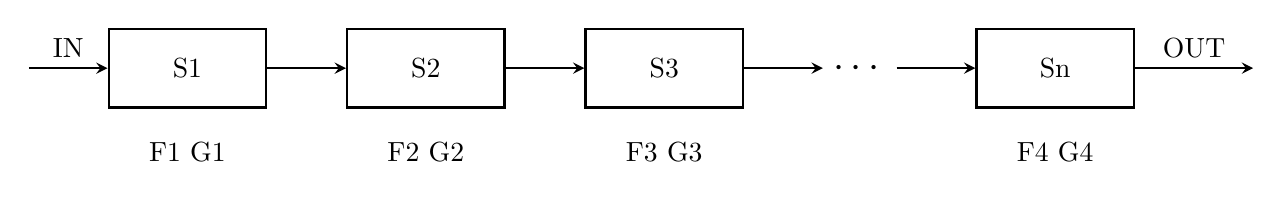
\begin{tikzpicture}[auto,thick,node distance=1cm,>=stealth]
      \tikzstyle{block}=[draw,rectangle,minimum height=1cm,minimum width=2cm]

      \node[block] (A) {S1};
      \node[block,right = of A] (B) {S2};
      \node[block,right = of B] (C) {S3};
      \node[right=of C] (dots) {\Large $\cdots$}; 
      \node[block,right = of dots] (D) {Sn};

      \node[below=0.3cm of A]{F1 G1};
      \node[below=0.3cm of B]{F2 G2};
      \node[below=0.3cm of C]{F3 G3};
      \node[below=0.3cm of D]{F4 G4};

      \draw[->] ([xshift=-1cm]A.west)--node[above]{IN}(A.west);
      \draw[->] (A)--(B);
      \draw[->] (B)--(C);
      \draw[->] (C)--(dots);
      \draw[->] (dots)--(D);
      \draw[->] (D.east)--node[above]{OUT}([xshift=1.5cm]D.east);
    \end{tikzpicture}\\
    等价于\\ \\
    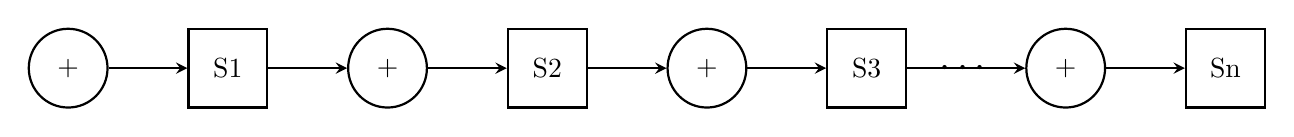
\begin{tikzpicture}[auto, thick, >=stealth, node distance=1cm]
      \tikzstyle{block}=[draw, rectangle, minimum height=1cm, minimum width=1cm]
      \tikzstyle{plus}=[draw, circle, minimum size=1cm, inner sep=0pt]
    
      \node[plus] (P1) {+};
      \node[block, right=of P1] (S1) {S1};
      \node[plus, right=of S1] (P2) {+};
      \node[block, right=of P2] (S2) {S2};
      \node[plus, right=of S2] (P3) {+};
      \node[block, right=of P3] (S3) {S3};
      \node[plus, right=of S3, xshift=0.5cm] (P4) {+};
      \node[block, right=of P4] (Sn) {Sn};
    
      \node at ($(S3)!0.5!(P4)$) {\Large$\cdots$};
    
      \draw[->] (P1) -- (S1);
      \draw[->] (S1) -- (P2);
      \draw[->] (P2) -- (S2);
      \draw[->] (S2) -- (P3);
      \draw[->] (P3) -- (S3);
      \draw[->] (S3) -- (P4);
      \draw[->] (P4) -- (Sn);
    \end{tikzpicture}
\end{enumerate}
\end{document}